\chapter{Literature Review}
\label{chap2}

\section{Introduction}

In this chapter, previous work and research findings relevant to this project are mentioned and discussed. These fields include the quadcopter platform, computer vision and machine learning techniques. Some concepts and terminology used in later chapters of this document are also explained and expanded upon.

\section{Quadcopters}

A quadcopter is an autonomous aerial vehicle (UAV) in a four-arm frame configuration. The frames typically come in an X or plus (+) shape with the control equipment and sensors located at the centre of the frame. Refer to Figure~\ref{fig:chap2-quad} for a picture of the Solar Thermal Energy Research Group's (STERG) Suncopter research platform which has an X configuration. They can also come equipped with either four or eight motors and props, though the four-rotor variant is commonly used and is used in this project.

\begin{figure}
  \centering
  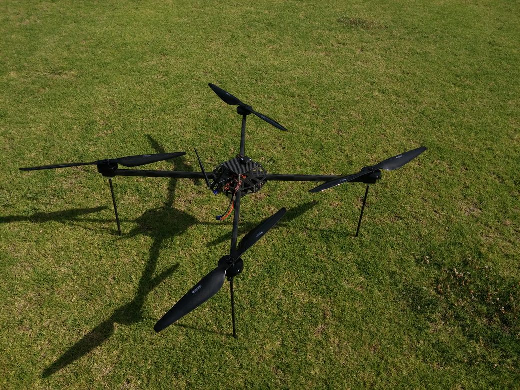
\includegraphics[clip, trim = 0 0 30 20, width=0.5\textwidth]{figures/chapter2/quadcopter}
  \caption[A picture of the Suncopter used by STERG.]{A picture of the Suncopter used by STERG.}
\label{fig:chap2-quad}
\end{figure}

Quadcopters move freely in three-dimensional space and have six degrees of freedom: three in position space ($x, y, z$) and three in orientation space ($\theta, \phi, \psi$), where the orientation is defined by the Eulerian aeroplane angle scheme, i.e.\ roll, pitch and yaw angles. The rotors on each axis of the frame rotate in the same direction and each axis' rotors spin in opposite directions relative to one another. Refer to Figure~\ref{fig:chap2-quad-rotation} for a diagram demonstrating this. 

\begin{figure}
  \centering
  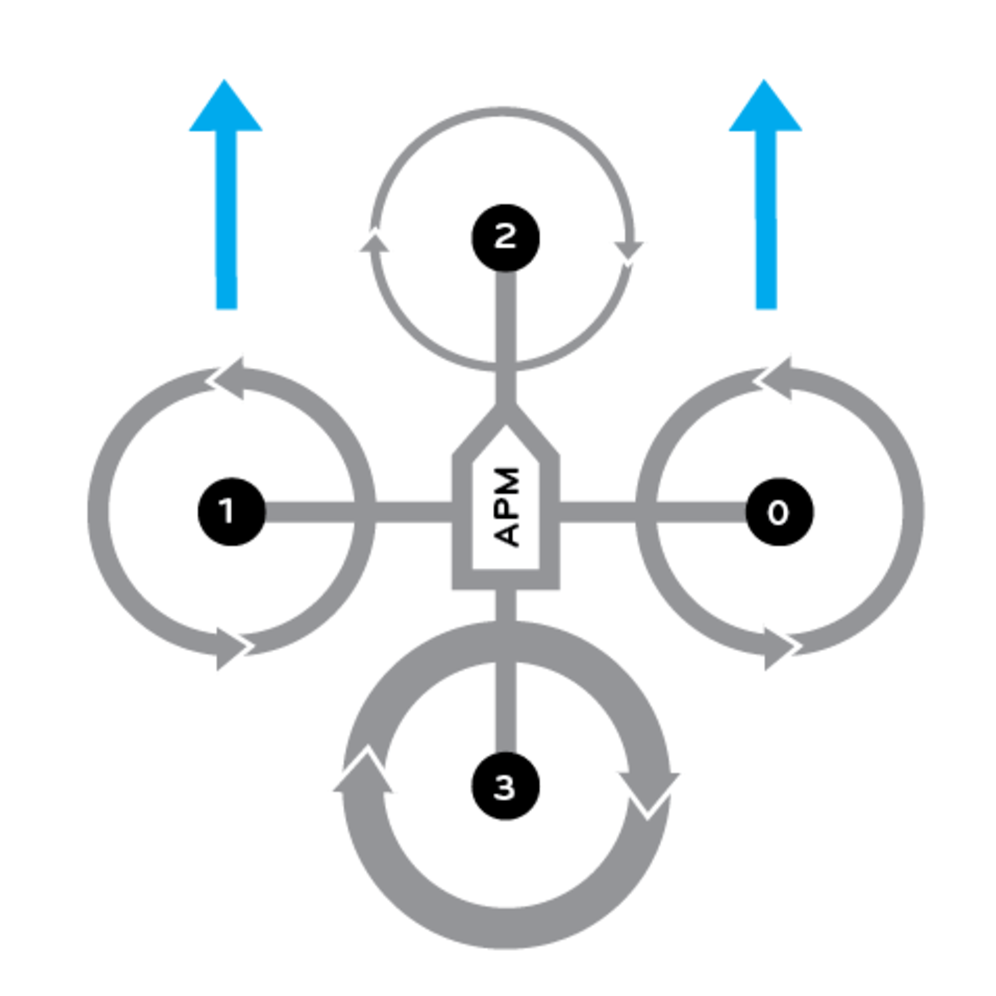
\includegraphics[width=0.5\textwidth]{figures/chapter2/quad_axis.pdf}
  \caption[Diagram presenting the opposing axis rotations directions.]{A diagram presenting the opposing axis rotation directions. The thickness of the arrows represent the power output of the motor~\citep{quad-rotation-pic}.}
\label{fig:chap2-quad-rotation}
\end{figure}

Movement in each of the six dimensions is described below. 

\begin{enumerate}
  \item Forward/backward or left/right movement: Keep one axis' rotor speed constant, while raising or lowering the speed of the rotors on the other axis (shown in Figure~\ref{fig:chap2-quad-rotation}).
  \item Higher/lower: Increase or decrease all of the rotor speeds.
  \item Roll/pitch: Linear movement is achieved by tilting the quadcopter, therefore movement in the roll and pitch dimensions is achieved with the same process as described in the first point. 
  \item Yaw: Increase or decrease the rotor speed of one axis relative to the other. 
\end{enumerate}

As described in Chapter~\ref{chap1}, the goal of this project is to determine a quadcopter's pose estimation error, i.e.\ the difference between a quadcopter's true pose and its estimated pose. To be able to do this, it is important that the dynamics and control strategies of a typical quadcopter are well defined and understood. This section sets out to discuss the work that has gone into the dynamic modelling of a quadcopter, as well as the different control strategies that have been developed and implemented in the past. 

\subsection{Quadcopter Modelling}

When designing a control system, arguably the most crucial part of the design process is to derive an accurate mathematical model of the plant, since an accurate plant model will lead to more stable response and superior performance. The plant in this case is a UAV in a quadcopter configuration. 

As part of their X-4 Flyer project,~\cite{hamel2002dynamic} set out to derive a simple model for their plant using only rigid body dynamics and abstract force and torque actuators. As stated by~\cite{Pounds2010c}, this model (like many others that were derived at the time) represents the quadcopter as a rigid body mass with inertia and autogyroscopics, which is only affected by gravity and actuator torques.~\citeauthor{Pounds2010c} further argue that these simple quadcopter models do not accurately represent the complex helicopter-like behaviour exhibited by real quadcopters at high rotor speeds. The high-speed rotor effects include blade flapping effects, which affect the quadcopter frame's oscillatory modes, rotor flapping introduced by varying a quadcopter's yaw angle and variable airflow velocities over the rotor blades caused by changing roll and pitch angles.

In an attempt to create a more accurate quadcopter model that will allow a quadcopter to be more controllable at high rotor speeds,~\citeauthor{Pounds2010c} set out to derive a model incorporating rigid body dynamics as well as the aerodynamic effects mentioned earlier. Their model is based, in part, on the diagram given in Figure~\ref{fig:chap2-quad-model}.

\begin{figure}
  \centering
  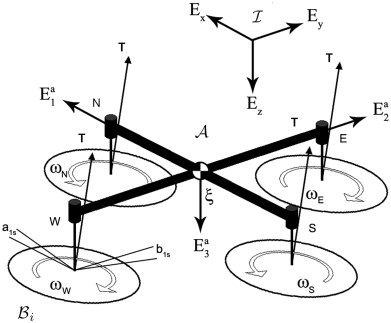
\includegraphics[width=0.5\textwidth]{figures/chapter2/pounds_quad-model.jpg}
  \caption[Diagram of the quadcopter model.]{A diagram of the quadcopter model which includes the blade flapping dynamics discussed by~\cite{Pounds2010c}.}
\label{fig:chap2-quad-model}
\end{figure}

Their resulting model was used to develop a simple Proportional Integral Differential (PID) attitude and altitude controller for the purpose of model verification. Their results show that the quadcopter stabilised itself (in indoor flight) with a level of precision of $\pm\ang{1}$, and $\pm\ang{5}$ during outdoor flight. The lower precision during outdoor flight is due to the added wind disturbances and sensor drift. They therefore conclude that their model is sufficiently accurate to safely control a quadcopter for hovering. However, they did not compare their more complex model against the model of~\citeauthor{hamel2002dynamic}, which is based solely on rigid body dynamics. 

\subsection{Control Strategies}

After an accurate model has been established, the next important part of designing a good control system is the controller itself. Many controllers have been implemented and tested on quadcopters over the years and different control strategies have also been investigated. Some of the most prevalent control strategies and controllers are discussed here.

\subsubsection{Indoor vs. Outdoor Control}

There are different types of quadcopters, with each of them equipped with different sensors and equipment. However, two types of quadcopters with distinctly different sensor and control approaches are relevant to this project. These are indoor and outdoor quadcopters and each of them work in different ways and implement very different control schemes. 

To help with stability control, indoor quadcopters may or may not come equipped with an on-board inertial measurement unit (IMU), which typically includes an accelerometer and a gyroscope. However, they commonly solely rely on an external motion detection system which tracks the quadcopter's movement and provides position and orientation feedback to the controller, thereby closing the control loop. These quadcopters can be very accurate due to the highly accurate external motion sensing equipment which are capable of sub-millimetre levels of accuracy~\citep{richards1999measurement}. As a result they are capable of performing remarkable acrobatic feats. However, these systems are restricted to carefully regulated and controlled indoor environments.

Outdoor quadcopters do not have the luxury of highly accurate external motion tracking systems and have to rely on their on-board sensors to provide the controller with pose feedback. A quadcopter's on-board sensor suite may vary between quadcopter platforms; however, they almost certainly come equipped with an IMU to provide pose data, but since the IMU readings for position data drifts with time due to integration errors, a GPS sensor is added to provide a base-line reading of a quadcopter's position. Other sensors that may be included are magnetometers, barometers, visual feedback sensors and sonar sensors. To combine the readings of the different sensors a filtering technique, such as an Extended Kalmann Filter, can be used. The pose estimation error of the combination of the different readings are, in theory, less than the most accurate sensor in the suite, but this has not yet been proven and the exact error margin is yet to be determined. 

\subsubsection{Hover Control}

Hover control refers to a quadcopter's ability to hover and remain stable at a set point in three-dimensional space. The stable hovering of a quadcopter has been the focus of many projects and research papers in the past 15 years. As a result, many different control methods and schemes have been investigated, implemented and compared. 

\cite{bouabdallah2004pid}, as part of their OS4 project, compared the modern linear quadratic regulator (LQR) and classic PID controller, with respect to the control performance (disturbance rejection, reference tracking, etc.) of a quadcopter.

They found that the PID controller produced better results than the LQR in terms of reference tracking and dynamic performance. This is a surprising result, since LQR controllers normally excel at controlling an unstable, underactuated plant such as a quadcopter platform. They suspect that the reason for this surprising result is that they neglected the effects of actuator dynamics, such as blade and rotor flapping, in their quadcopter model and the PID was better at handling plant uncertainties. They expect that an LQR controller will outperform a PID controller if a more accurate model is used which takes aerodynamic effects into account. 

Some researchers have also investigated controlling a quadcopter using an H-infinity (H$_{\inf}$) control structure and a model predictive controller (MPC). Most notably,~\cite{raffo2010integral} have done extensive research on this topic. MPCs are modern computationally efficient controllers that drive a plant's state to a reference state within predefined constraints (eg.\ motor saturation, model dynamics, etc.), while a properly designed, non-linear H$_{\inf}$ controller is very good at rejecting disturbances (eg.\ wind gusts, motor vibrations, etc.) and are robust to model uncertainties. They opted to combine the two controllers in an intelligent manner to extract the best performance from their quadcopter. 

In their simulations, they found that the resulting controller exhibited good performance characteristics; presenting good reference tracking, proving to be robust with uncertain mass and inertia terms and deals well with disturbances on all six degrees of freedom at different points in time. However, they are yet to implement their controller configuration on a real quadcopter. Although the algorithms and methods they used are computationally efficient, it may still prove to be too computationally intensive for the limited computing power on-board a UAV.\@ Given the fast growth of processing power, however, this controller configuration may become a more viable option in the near future. 

Controllers for enabling a quadcopter to hover have already been successfully designed and implemented, and it is therefore possible to stabilise and accurately control a quadcopter for hovering operations. 

\section{Computer Vision}

Computer vision is a diverse field which primarily focuses on finding methods for acquiring, processing, analysing and understanding images captured of the world. The `world' in this context refers to the three-dimensional world as perceived by living beings. There are many sub-fields of research, but a common theme across all of them is to make a computer mimic the human ability to perceive and understand an image and elicit an appropriate response to different visual inputs. 

The fields of interest for this project are feature detection, feature tracking and pose estimation. This section discusses the work that has been performed in these fields of research.  

\subsection{Camera Matrix}

A digital image is a collection of two-dimensional colour intensity vectors representing a collection of three-dimensional space vectors. These collections of vectors are related by a matrix, $C$, known as the camera matrix. The camera matrix contains the intrinsic parameters of the camera that recorded the image, i.e.\ the focal lengths and principle point of the camera, as well as the extrinsic, or pose, parameters of the camera, i.e.\ the camera's position and orientation information. The camera matrix, $C$, as derived by~\cite{heikkila1997four}, is 

\begin{equation}
  \label{eq:chap2-cam-matrix}
  C = 
  NP.
\end{equation}
The matrix $N$ in Equation~\ref{eq:chap2-cam-matrix} is given by

\begin{equation}
  \label{eq:chap2-cam-intrinsic}
  N = 
  \begin{bmatrix}
    f_x & 0   & u_0 \\
    0   & f_y & v_0 \\
    0   & 0   & 1   \\
  \end{bmatrix}.
\end{equation}
Here, $f_x$ and $f_y$ describe the focal lengths of the camera, while $u_0$ and $v_0$ represent the camera's principal point coordinates. The principal point, also known as the focal point, is where the camera's axis crosses the image plane and is ideally situated in the centre of the camera lens. However, due to manufacturing defects, this is rarely the case. Refer to Figure~\ref{fig:chap2-focal} to see what the focal length and principle point coordinates represent. 

\begin{figure}
  \centering
  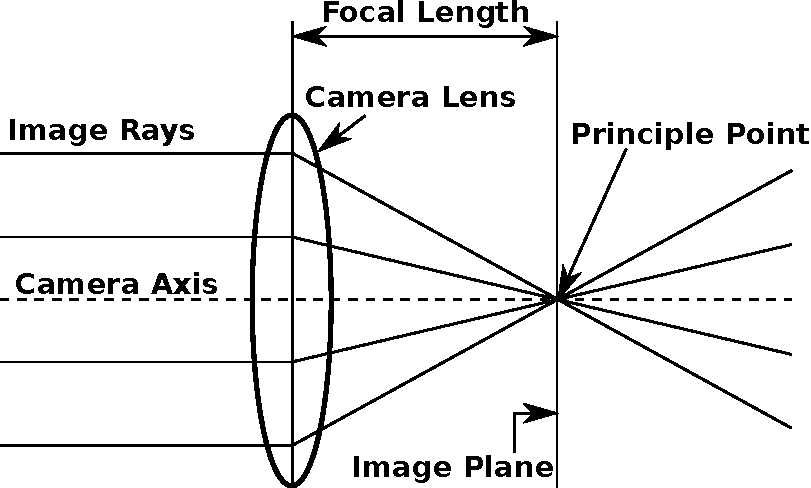
\includegraphics[width=0.6\textwidth]{figures/chapter2/focal_details}
  \caption{Diagram showing what the focal length and principle point parameters represent. }
\label{fig:chap2-focal}
\end{figure}

The pose matrix, $P$, from Equation~\ref{eq:chap2-cam-matrix} is given by

\begin{equation}
  \label{eq:chap2-cam-extrinsic}
  P = 
  \begin{bmatrix}
    R | \bm{T}
  \end{bmatrix}
  =
  \begin{bmatrix}
    r_{11} & r_{21} & r_{31} & t_1 \\
    r_{21} & r_{22} & r_{32} & t_2 \\
    r_{31} & r_{23} & r_{33} & t_3 \\
  \end{bmatrix}.
\end{equation}
In the matrix $P$, $R$ is a $3\times3$ cell matrix describing the orientation of the camera and $\bm{T}$ is a three-dimensional vector describing the position of the camera. The pose information in $P$ is given relative to some reference object or plane. 

The two-dimensional image projection of an object in three-dimensional world space is related through $C$ with the relation given in Equation~\ref{eq:chap2-2d-to-3d}. The camera matrix is commonly determined through some camera calibration procedure. One such a procedure is discussed in Section~\ref{sec:chap2-cam-calibration}.

\begin{equation}
  \label{eq:chap2-2d-to-3d}
  \bm{x}_c
  = C
  \bm{X}_w
\end{equation}
In Equation~\ref{eq:chap2-2d-to-3d}, $\bm{x}_c$ is a homogeneous image vector $[x\;y\;1]$ and $\bm{X}_w$ is a homogeneous world coordinate vector $[X\;Y\;Z\;1]$. 

\subsection{Camera Calibration}
\label{sec:chap2-cam-calibration}

A properly calibrated camera is an important part of any computer vision system, since the accuracy of the data extracted from an image strongly depends on the accuracy of the calibration procedure and results. The goal of the calibration procedure is to produce the matrix $C$ (as given in Equation~\ref{eq:chap2-cam-matrix}), as well as finding the camera's distortion coefficients introduced by low-quality or fish-eye lenses. There are various camera calibration procedures available: from the two-step calibration described by~\cite{melen1994geometrical} to the classical approach given by~\cite{slama1980manual} where a non-linear error function is minimised. However, the minimisation problem presented by~\citeauthor{slama1980manual} is computationally inefficient and slow, while~\citeauthor{melen1994geometrical}'s method does not account for image distortion and correction. A popular calibration method is the four-step method proposed by~\cite{heikkila1997four} as an extension to the two-step method which was the prevalent calibration procedure at the time.

The \emph{calibrateCamera()} function of the OpenCV\footnote{Open-source computer vision library, OpenCV v2.4.8. Source-code available at github.com/Itseez/opencv} computer vision library \citep{bradski2000opencv} makes use of the four-step method. The details of this method is beyond the scope of this research project, however, a broad overview of the steps and equipment required to calibrate a camera is provided. 

To perform the calibration and find the camera matrix, OpenCV requires two sets of data: one two-dimensional image data set, $\bm{x}_c$, as well as a set of corresponding three-dimensional data points, $\bm{X}_w$. This implies that image data of an object, where the dimensions and coordinates of certain features are known, must be recorded. In practice, any well-characterised object can be used for calibration. For example, some calibration methods rely on a three-dimensional cube covered in precisely laid out markers. However, since manufacturing and distributing such precisely constructed objects to a large audience is infeasible, OpenCV opts to use a more convenient flat, regular pattern, such as chessboard or asymmetrical dot pattern. Figure~\ref{fig:chap2-calib-pattern} shows an example of a typical chessboard pattern generated by OpenCV.\@ With this flat pattern, the features used to populate the data sets would be the corners on the chessboard, i.e.\ where one black block meets another black block. The drawback to this approach, however, is that multiple views of the flat calibration pattern are required, whereas a single image of a three-dimensional object would suffice. However, more data points would allow the optimisation procedure built into the algorithm to find a more accurate result.  

\begin{figure}
  \centering
  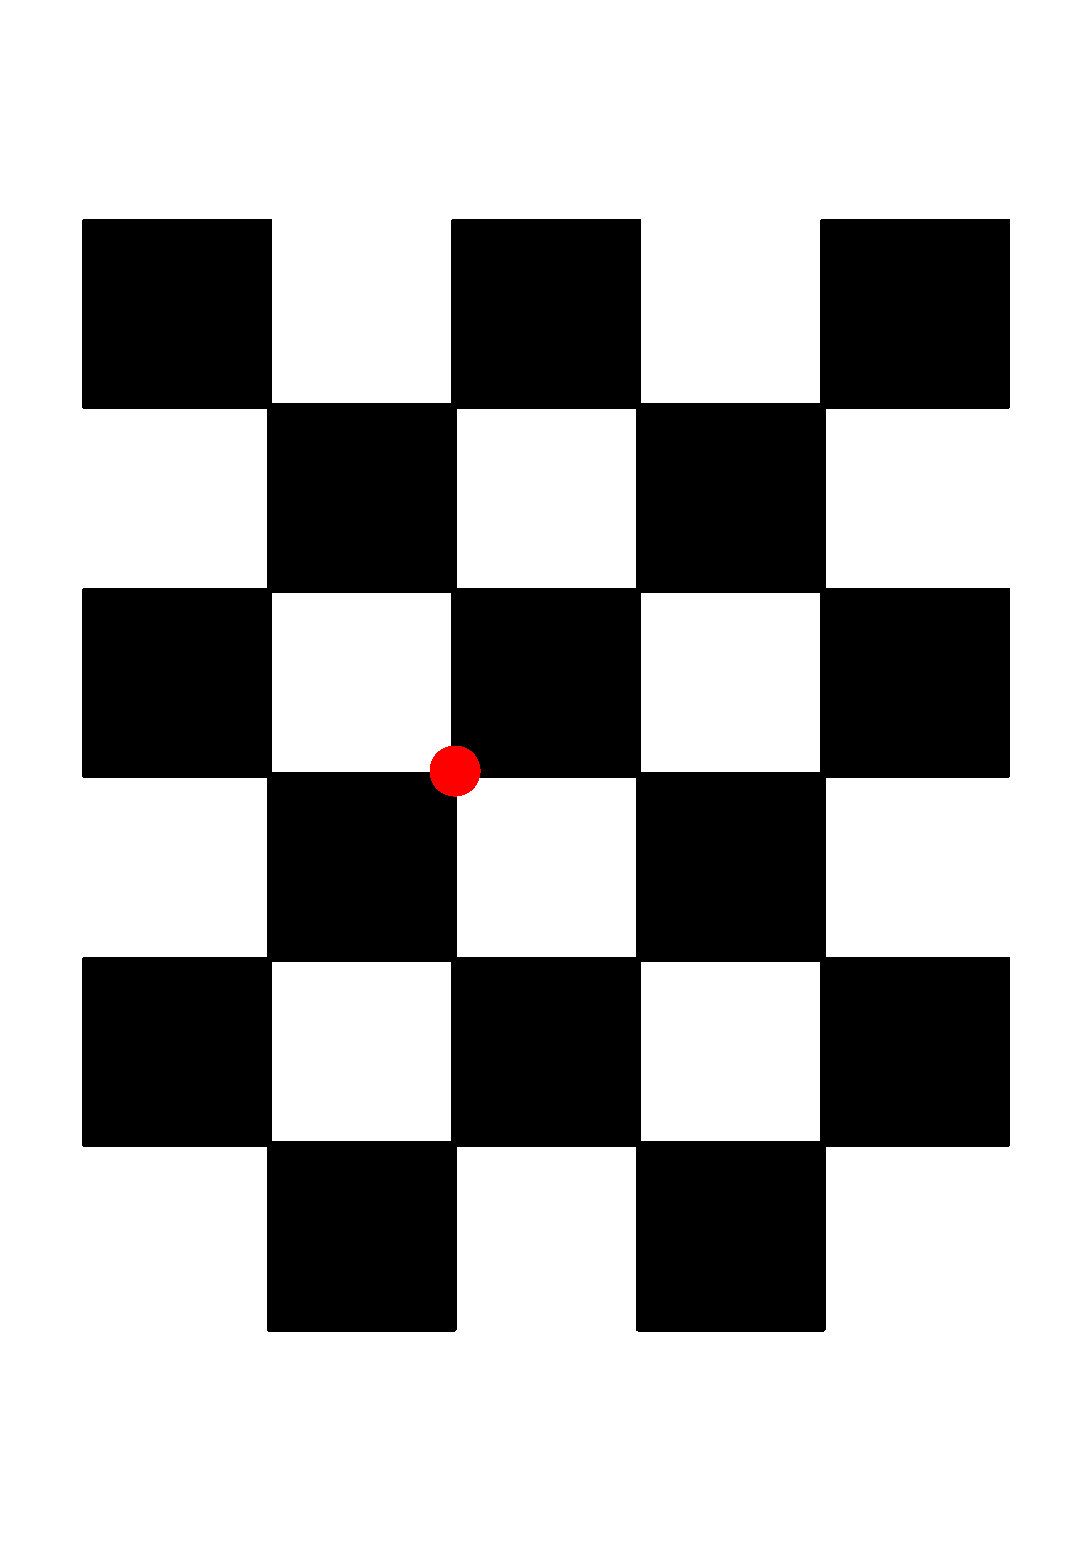
\includegraphics[angle=90, width=0.5\textwidth]{figures/chapter2/chessboard_pattern}
  \caption{An example of a typical chessboard pattern used for calibration.}
\label{fig:chap2-calib-pattern}
\end{figure}

In the case of the chessboard pattern, acquiring the two-dimensional pixel coordinates of the corners is accomplished by using OpenCV's \emph{findChessboardCorners()} and \emph{findCornerSubPix()} functions, which make use of the corner detection algorithm described by~\cite{harris1988combined}. The three-dimensional world coordinates of the features are fed into the calibration function according to an axis-system and measurement unit defined by the programmer. These coordinates can be as simple as a vector containing the feature coordinates in square units, where, for example, the corner from Figure~\ref{fig:chap2-calib-pattern} will be represented as $(3, 2, 0, 1)$ in homogeneous coordinates (note that $z$ will be zero since the board is flat). 

For the best calibration results, OpenCV recommends that camera calibration takes place within a well-lit room with a white background, using a calibration pattern with a wide white border in clear view of the camera and at different positions and orientations relative to the camera. These recommendations are mainly to increase the contrast between the black features and the white background on the calibration pattern and make it easier for OpenCV to accurately find each feature's pixel coordinates. Furthermore, the more diverse the position and orientation data is, the more accurate the estimate for the intrinsic camera parameters will be. 

Once the two-dimensional and three-dimensional data sets are known, Open\-CV's \emph{calibrateCamera()} function can determine the camera matrix, $C$. 

\subsection{Principle n-Points Problem}

The Principle n-Points (PnP) problem, as stated by~\cite{horaud1989analytic}, `is the problem of finding the position and orientation of a camera with respect to a scene object from $n$ correspondence points', where the scene object would normally be a well-characterised calibration object or pattern. It is a well-researched sub-field of computer vision with different solutions to the problem that have been proposed. They include some non-iterative solutions, such as the P3P solution proposed by~\cite{gao2003complete} and the PnP solution by~\cite{lepetit2009epnp} and~\cite{schweighofer2006robust}, and iterative solutions such as the method proposed by~\cite{lu2000fast}.

It was found that iterative methods produce very accurate results, but can become unstable if it is not properly initialised and can take a long time to converge. Conversely, the non-iterative ePnP method by~\citeauthor{lepetit2009epnp} implements~\citeauthor{schweighofer2006robust}'s robust solver and produces results whose accuracy is comparable to those produced by its iterative counterpart. However, it produces these results in a fraction of the time, having a big-$\mathcal{O}$ complexity that grows linearly ($\mathcal{O}(n)$), as opposed to competing non-iterative methods which commonly have a big-$\mathcal{O}$ complexity in the order of 4 or more ($\mathcal{O}(n^4)$). Unfortunately, the accuracy of the ePnP method's results are fairly dependant on the number of sample points, i.e.\ the number of feature correspondences between the three-dimensional features and their two-dimensional projections. 

The OpenCV library has implementations of both the P3P and ePnP methods, as well as its own solution based on Levenberg-Marquardt optimisation, as described by~\cite{levenberg1944method} and~\cite{marquardt1963algorithm}, where the pose that minimises the reprojection error - that is the sum of the squared distances between the actual two-dimensional points and the projected two-dimensional points - is determined and selected~\citep{opencv-levenberg}. 

OpenCV's \emph{solvePnP()} function can be used to determine the pose of a camera relative to a calibration pattern. This can be accomplished as follows. During the camera calibration procedure, the intrinsic parameter matrix, $N$, of Equation~\ref{eq:chap2-cam-intrinsic} is determined. Then, using a calibration pattern, a set of three-dimensional feature coordinates and their corresponding two-dimensional projection is obtained. Following from Equation~\ref{eq:chap2-2d-to-3d}, with the matrix $C$, the two-dimensional image projection vector, $\bm{x}_c$, and the three-dimensional object coordinate vector, $\bm{X}_w$, the pose matrix, $P$, can be found. This matrix contains the position and orientation data for the camera relative to the calibration pattern. 

\subsection{Random Sample Consensus}

For both the camera calibration and PnP solving functions, two-dimensional image projection data of a three-dimensional object is required. As mentioned, OpenCV's \emph{findChessboardCorners()} function can automatically detect corner features on a chessboard pattern and provide the two-dimensional projection data. However, the methods employed are prone to erroneously classifying some features as corners, introducing unwanted noise into the system. 

To remedy this,~\cite{fischler1981random} proposed a new algorithm to iterate through a data set and reject any outlier data. This algorithm is known as RAndom SAmple Consensus (RANSAC) and is commonly used in the computer vision field to determine if an image feature, e.g.\ a corner on a chessboard, has been classified correctly and rejecting it if it was not, thereby reducing the amount of noise in a data set. 

\section{Machine Learning}

Machine learning is a research field in computer science with strong ties to the fields of mathematical statistics and optimisation. The field is well-es\-tab\-lished and has its roots with a paper by~\cite{turing1950computing} in which he poses the question, `Can machines think?'.~\cite{michalski2013machine} offers a somewhat more formal definition: `A computer program is said to learn from experience E with respect to some class of tasks T and performance measure P, if its performance at tasks in T, as measured by P, improves with experience E'. This means that researchers in the machine learning field are attempting to find efficient methods and algorithms that will allow a computer to be trained to make intelligent decisions when presented with an arbitrary input data set. 

An everyday example of a system that uses machine learning is the face detection software that often come packaged with digital cameras. Here, the camera has been trained to search for facial information within the image, and consequently detects them when presented with other images containing faces.

Various machine learning algorithms and types have been developed, each of them having their unique advantages and limitations. Here, brief discussions on the most prevalent machine learning methods are provided. 

\subsection{Artificial Neural Networks}

Artificial neural networks (ANNs) are a family of machine learning algorithms which have seen a rise in popularity in recent years. The idea behind ANNs is to model the vast network of interconnected neurons in a biological brain in such a way that the network can be trained to recognise patterns and make decisions based on what it perceives, much like any animal or human would. 

Normally, an ANN consists of a multitude of artificial `neurons', or nodes, numbering anything between a handful to many millions, arranged in a series of layers. Each of the nodes in every layer is connected to each other node in the layers on either side of it, forming a vast network of interconnected nodes forming something analogous to a living brain. A diagram of the layout of a simple feed-forward ANN is given in Figure~\ref{fig:chap2-ann-layout}.

\begin{figure}
  \centering
  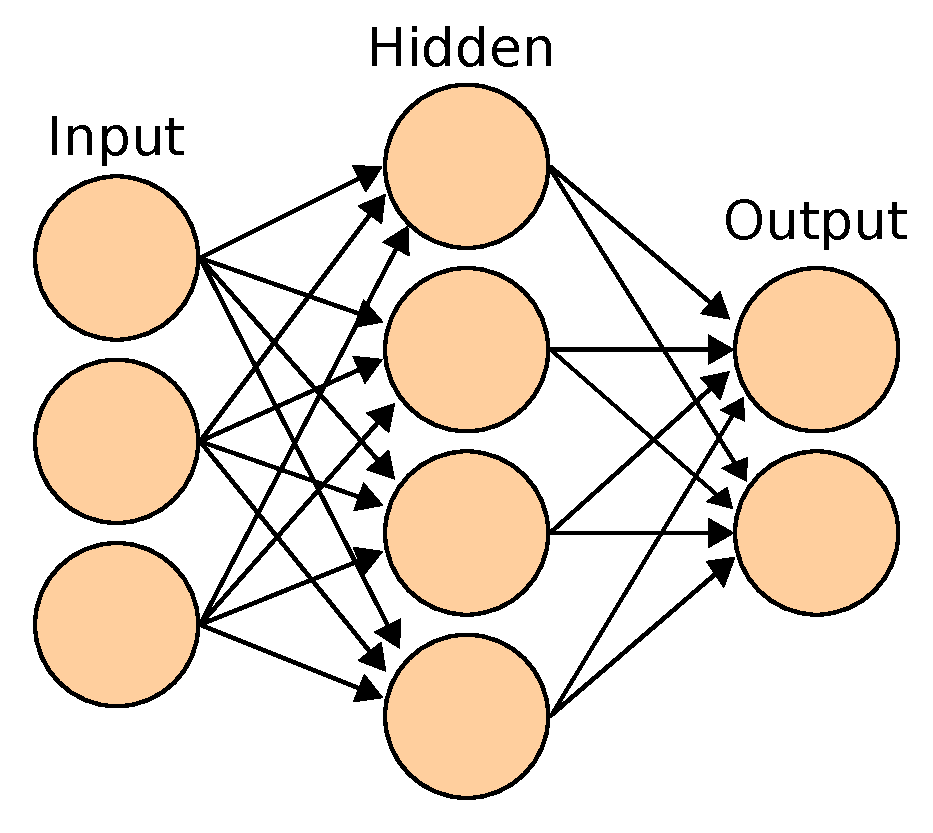
\includegraphics[width=0.5\textwidth]{figures/chapter2/ANN_diagram}
  \caption[Diagram of a simple ANN.]{Diagram of a simple ANN~\citep{ann-wiki-pic}.}
\label{fig:chap2-ann-layout}
\end{figure}

Each network has two special layers called the input and output layers. The input layer accepts information from which the ANN's designer wants data extracted. The output layer is responsible for producing the output which contains the information on how the network responded to the input excitation data. In-between these extreme layers lie the so-called `hidden' layers. These layers form the majority of the network and are responsible for interpreting the input data and producing the network's output. 

The connections between the hidden nodes are represented by a weighting factor which are determined during a training process. These weights define how much influence the nodes have over another, i.e.\ if a weight is positive, it excites another node, whereas if it is negative, it suppresses the node. The input information traverses the hidden layers, activating the next node with the highest connection weighting. The output data is then determined by which of the nodes were traversed in the hidden layers. The connections between the hidden node layers are mostly responsible for the output and different connection schemes provide different performance characteristics. 

Consider a simple example: you wish to create an ANN to recognise whether a picture contains a man or a dog. You train it with 25 images of different men and dogs, telling the ANN which picture contains which. After it has been trained, you show it a picture containing a young boy which is totally unfamiliar to the network. Based on the way you trained it, the network should recognise enough human and male features in the child to come to the conclusion that it is more likely that the child is a man rather than it is being a dog. 

This ability to classify information that technically falls out of the network's training environment is one of the strengths of ANNs. This advantage, as stated by~\cite{tu1996advantages}, is ANNs' ability to implicitly detect any non-linear relationships between multi-dimensional input and output dimensions. They can also be trained using different training schemes and some modern software packages and libraries have also made it fairly easy to develop a model without any formal statistical training. Some drawbacks of ANNs are that they may require an immense amount of computing power if many nodes are initialised, they are prone to overfitting data when a poorly selected number of nodes are used and the trained models are extremely `black-box' solutions, making it difficult to identify and characterise the relationships between the nodes. 

Different ANN topologies and layouts, have been developed and proposed. Some of them are briefly discussed in the following sections.

\subsubsection{Feed-forward Network}

The oldest, and arguably the simplest ANN topography is the feed-forward network (FFN), also referred to as multi-layer perceptron if there are multiple layers in the hidden layer. Its layout is typically similar to the one given in Figure~\ref{fig:chap2-ann-layout}, with a single input and output layer, as well as a single or multiple hidden node layers. 

The FFN uses some form of supervised training algorithm, with the backpropagation algorithm commonly used. Here, the hidden nodes' weights are adjusted until the output the network produces is as close as possible to the target output specified by the designer. This configuration's biggest attractions are its simplicity, relatively fast training speed, depending on the number of hidden layers, and its ability to derive non-linear relationships between dimensions. However, FFN's are prone to converging very slowly and sometimes getting stuck in local minima, as stated by~\cite{svozil1997introduction}. However, improvements to the backpropagation training scheme have reduced this effect.

\subsubsection{Recurrent Neural Network}

The recurrent neural network (RNN) is a family of neural networks. The hidden nodes of an RNN make provision for feedback between the different hidden layers and the output layer, creating an internal state for the network. See Figure~\ref{fig:chap2-rnn-diagram} for a diagram of a RNN topography.

\begin{figure}
 \centering
 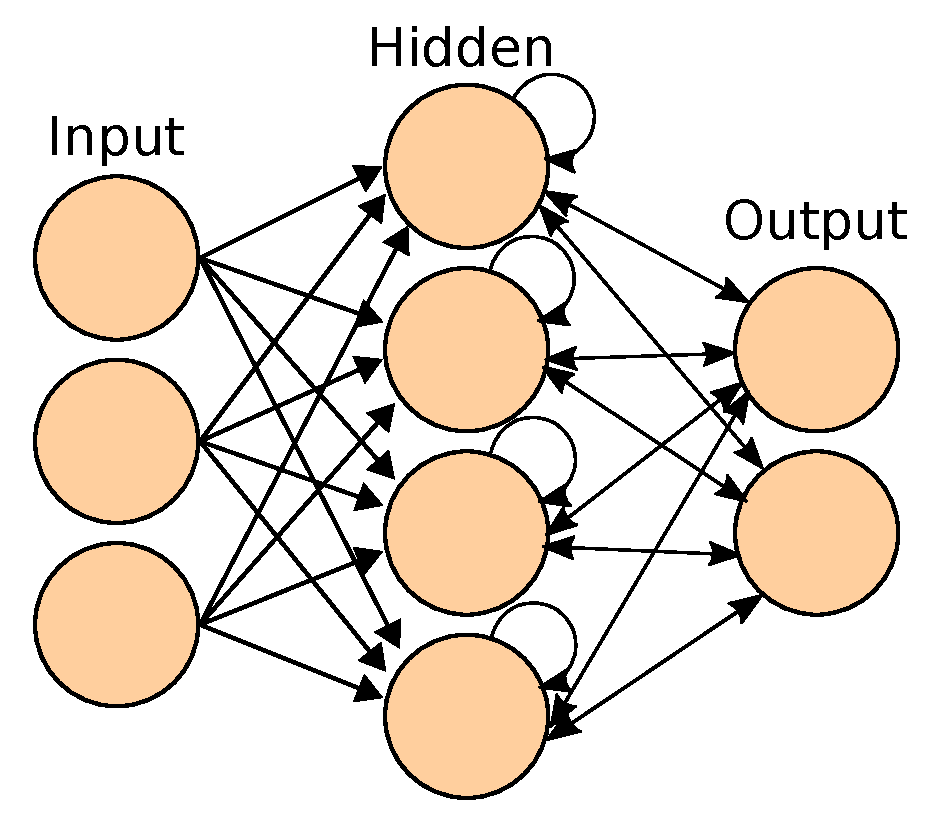
\includegraphics[width=0.5\textwidth]{figures/chapter2/rnn_diagram}
 \caption[Diagram of a simple RNN.]{A diagram of a simple RNN (adapted from~\citeauthor{ann-wiki-pic}, \citeyear{ann-wiki-pic}).}
\label{fig:chap2-rnn-diagram}
\end{figure}

In contrast to the FFN, this internal saved state allows the RNN to process arbitrary sequences of input data, making it adept at processing unsegmented speech or handwriting patterns. However, the added complexity of adding feedback loops between the different layers becomes computationally expensive, especially when large networks with many layers and inputs are used. Increases in computing power and improvements in the training process, as well as a better understanding of RNNs and ANNs in general, have alleviated the computational expense somewhat.

There are different RNN configurations available. These include the Hopfield network~\citep{hopfield1982neural}, the echo network~\citep{jaeger2001echo} and the recurrent multilayer perceptron network~\citep{tutschku1995recurrent}.

\subsubsection{Radial Basis Function Network}

The radial basis function neural network (RBFNN) is another type of neural network and is a sub-family of the RNN family, as stated by~\cite{wilamowski1996implementation}. 

The RBFNN topology is fixed to a three-layer architecture, with one input layer, one hidden layer and one output layer. The input layer provides the input. The hidden layer then remaps these inputs to make them linearly separable, where the output layer does the separation and outputs the data~\citep{xie2011comparison}.  

Despite belonging to the same family of ANN, there are a number of significant differences between the RBFNN and RNN.\@ Firstly, the three-layer RBFNNs are simpler than multi-layered RNNs, making the training process for RBFNNs generally faster than for an RNN.\@ Secondly, and most importantly, as stated by~\citeauthor{xie2011comparison}, is the difference in how the RBFNN and RNN classifies the data: the RBFNN data clusters are separated by a hyper sphere, whereas RNNs use arbitrarily shaped hyper surfaces. See Figure~\ref{fig:chap2-classifier} for a visualisation of these class separation strategies. This makes RBFNNs an attractive option to interpolate multidimensional data.

\begin{figure*}
  \centering
  \begin{subfigure}{0.5\textwidth}
    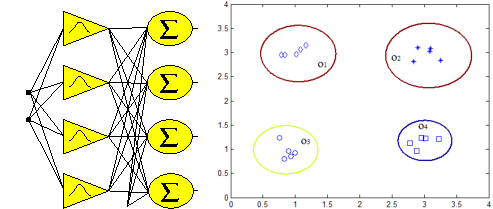
\includegraphics[width=\textwidth]{figures/chapter2/rbf_class}
    \caption{}
    \label{fig:chap2-rbf-classifier}
  \end{subfigure}
  \begin{subfigure}{0.5\textwidth}
    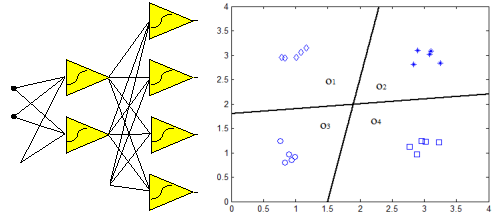
\includegraphics[width=\textwidth]{figures/chapter2/rnn_class}
    \caption{}
    \label{fig:chap2-rnn-classifier}
  \end{subfigure}
  \caption[Comparison between the RBF and RNN classifiers. ]{A comparison between the RBF classifier in Figure~\ref{fig:chap2-rbf-classifier} and the RNN classifier in Figure~\ref{fig:chap2-rnn-classifier} as shown by~\cite{xie2011comparison}. }
\label{fig:chap2-classifier}
\end{figure*}

\citeauthor{xie2011comparison} further determined that RBFNNs are well suited to interpolate noisy data where the data surfaces contain regular valleys and peaks. In contrast, normal ANNs and RNNs are more efficient for classification problems and for well-conditioned, regularly spaced data. 

As described by~\cite{skala2012radial}, the function on each node is given by 

\begin{equation}
  \label{eq:chap2-rbf}
  f(\bm{x}_i) = \sum\limits_{j = 1}^{M}\lambda_j \phi(|| \bm{x}_i - \bm{x}_j ||).
\end{equation}
Therein, $\lambda_j$ is the node weighting factor and $\bm{x}_j$ are the kernel centres which are determined during the model training phase. The function $\phi$ is the radial function of the euclidian norm of the distance between the node centre and the input vector. This radial function is variable and the designer can select the function which best describes the data, although a Gaussian radial function, i.e.\ $\phi(\bm{r}_{ij}) = e^{-(\frac{\bm{r}_{ij}}{\epsilon})^2}$, $\bm{r}_{ij} = || \bm{x}_i - \bm{x}_j ||$, is commonly used.  

\subsection{Support Vector Machines}

Support vector machines (SVM) is a widely used classification technique first proposed by~\cite{vapnik1995support}. It works by finding a hyperplane between two data classes that separates the classes by the widest possible average margin. See Figure~\ref{fig:chap2-svm-linear} for an illustration of this separation.

\begin{figure}
  \centering
  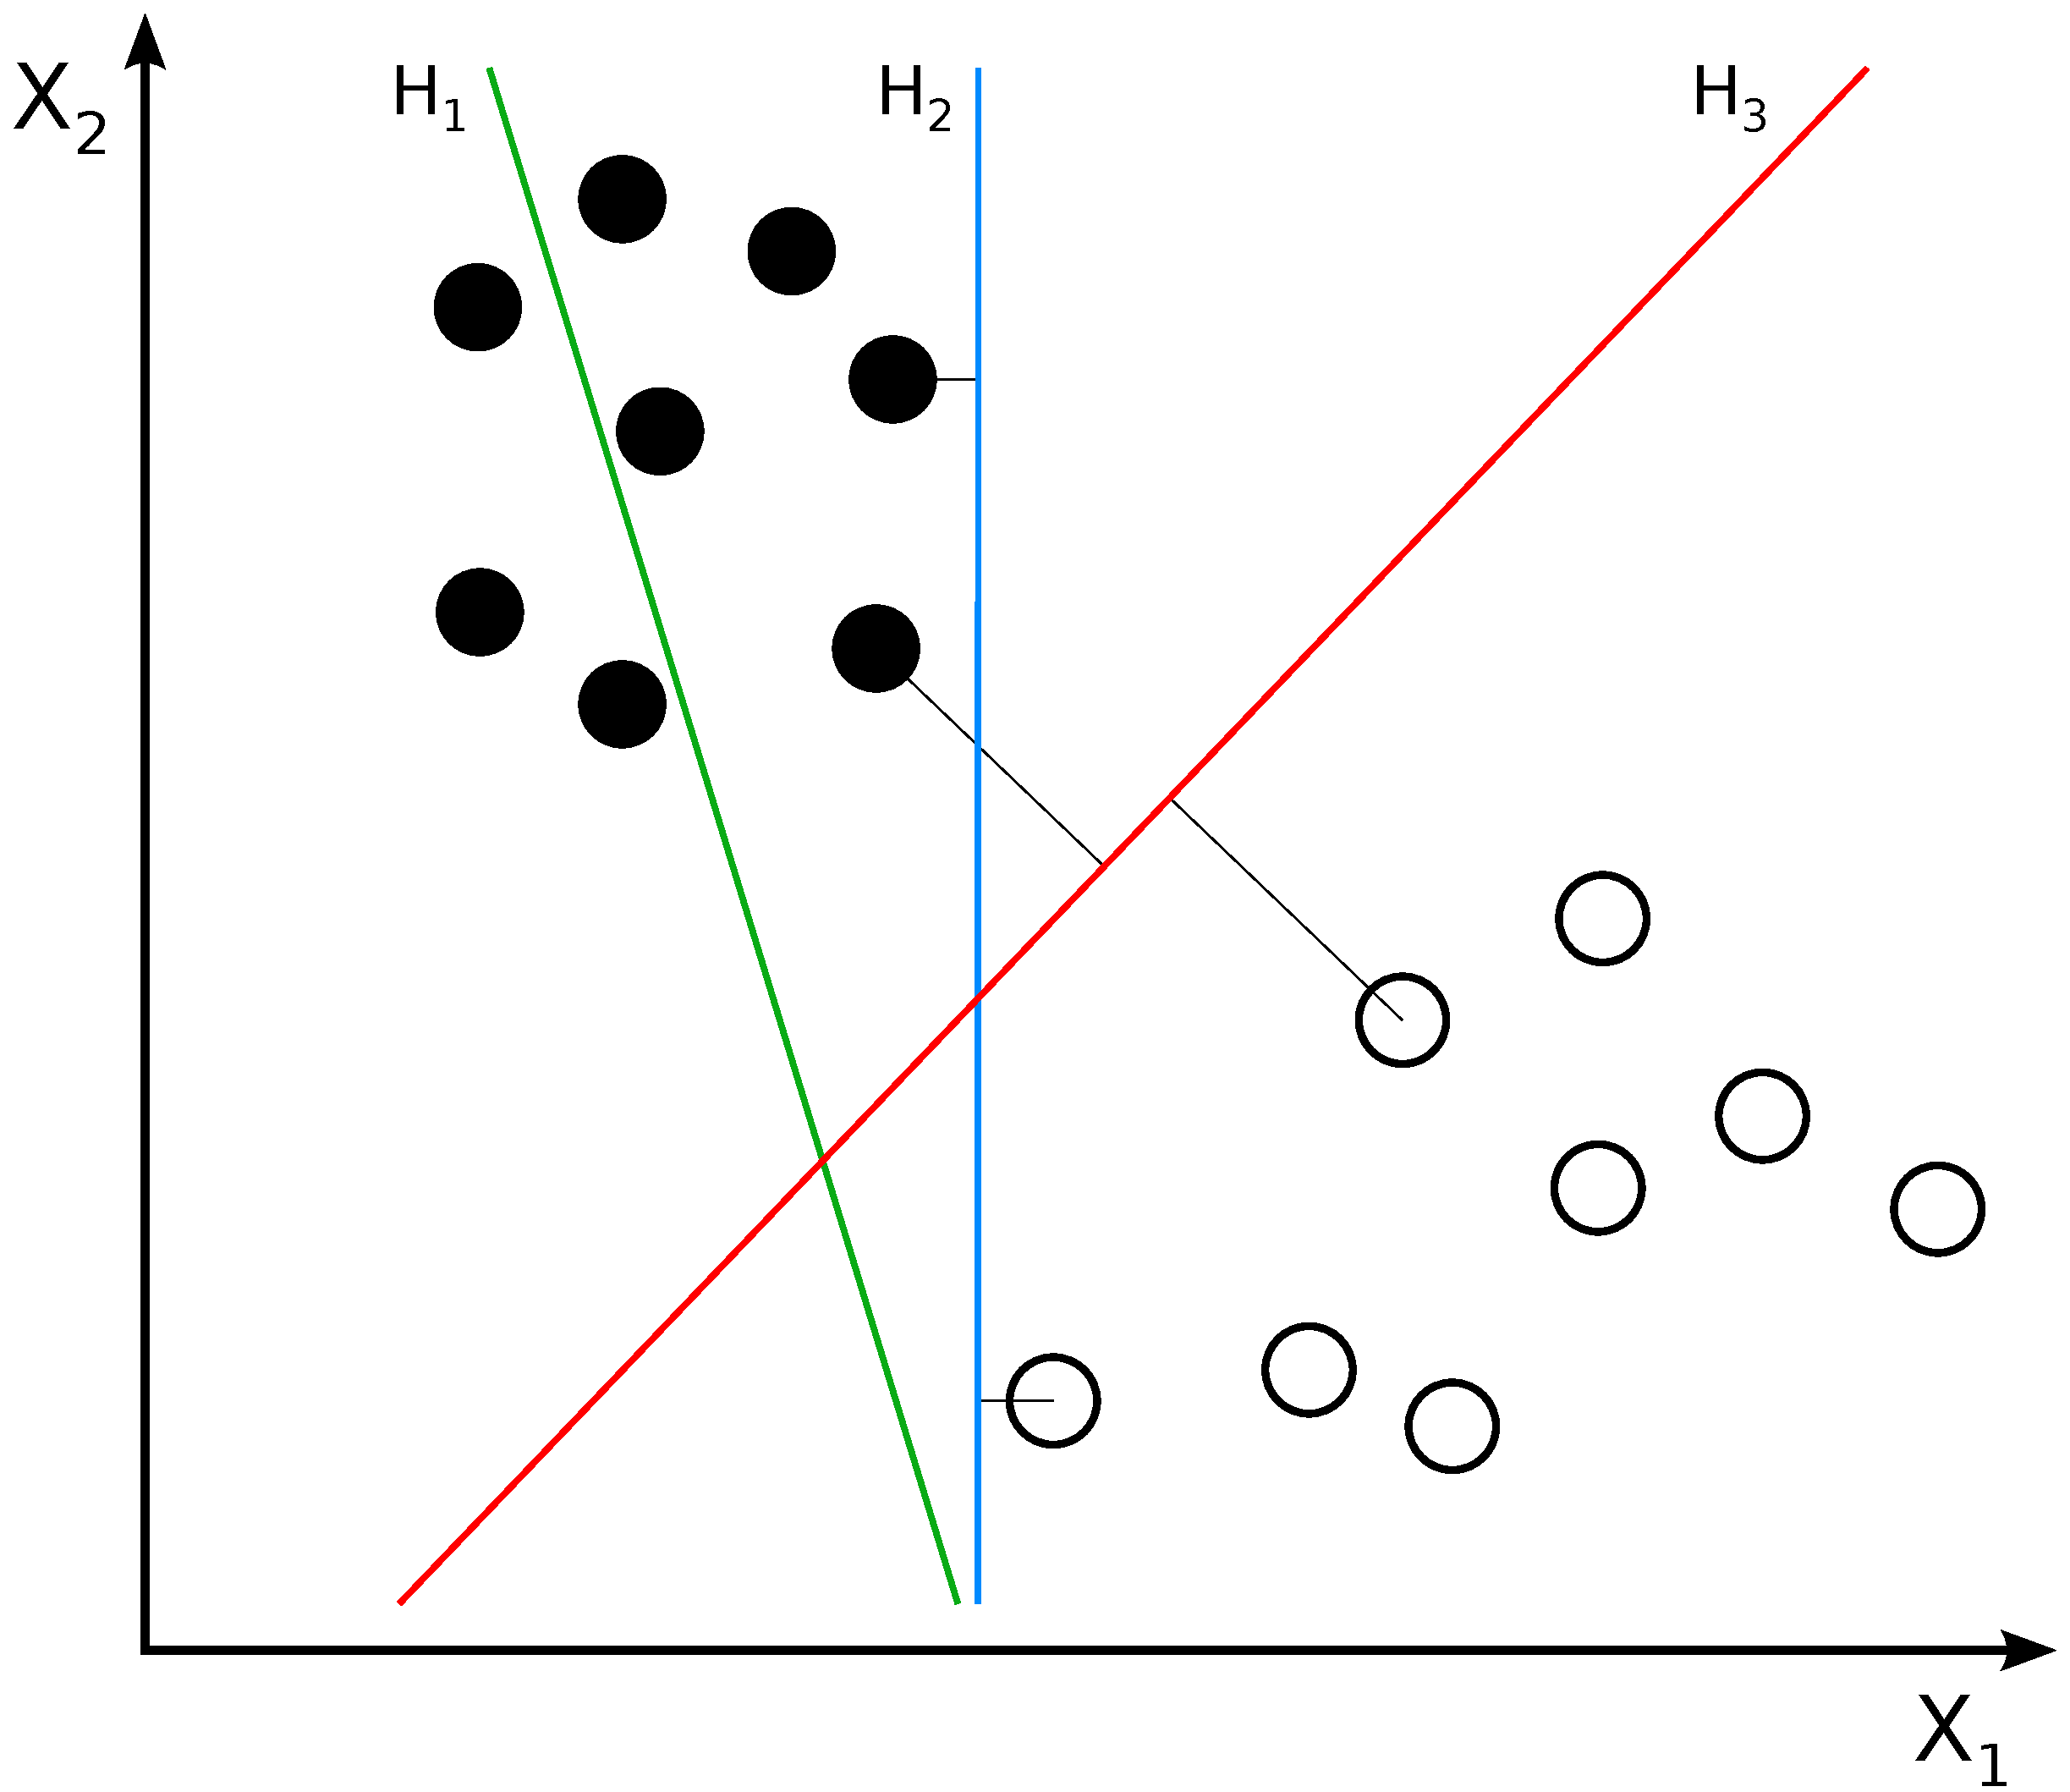
\includegraphics[width=0.5\textwidth]{figures/chapter2/svm_linear}
  \caption[SVM with a linear hyperplane.]{An SVM plot illustrating different class separators~\citep{svm-wiki-pic}.\@ $H_1$ does not separate the classes, while $H_2$ has only minimal class separation. $H_3$ exhibits the widest average separation margin.}
\label{fig:chap2-svm-linear}
\end{figure}

\citeauthor{vapnik1995support}'s original method was limited to linear hyperplanes. Since then, the algorithm has extended to non-linear hyperplanes by applying what is known as the `kernel trick', as described by~\cite{amari1999improving}. An example of such a non-linear separator can be seen in Figure~\ref{fig:chap2-svm-nonlinear}.

\begin{figure}
  \centering
  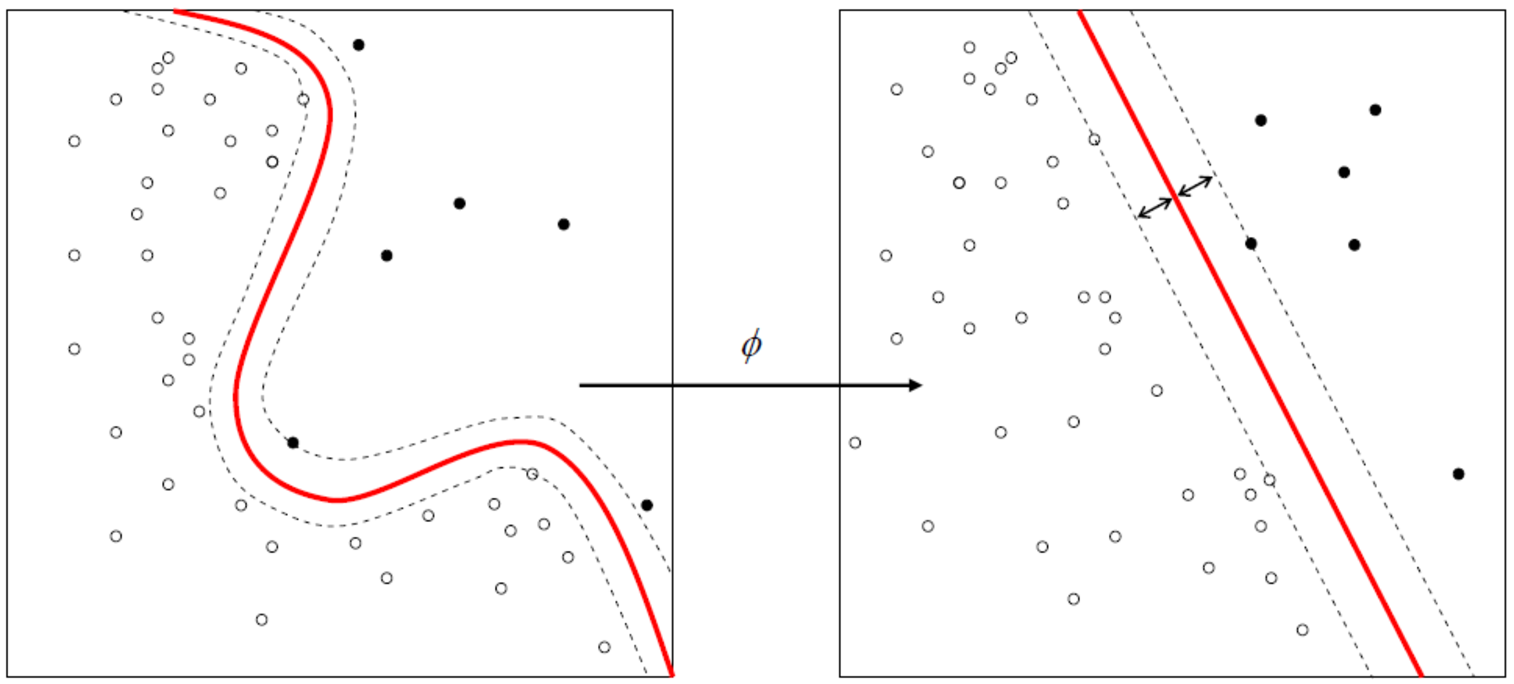
\includegraphics[width=0.8\textwidth]{figures/chapter2/svm_nonlinear}
  \caption[Example of an SVM with a non-linear kernel separator.]{An example of an SVM with a non-linear kernel separator~\citep{kernel-wiki-pic}.}
\label{fig:chap2-svm-nonlinear}
\end{figure}

SVM's are limited to  binary problems with two classes, somewhat limiting their potential for high-dimensional problems. Regardless, they are extremely popular in scientific circles due to their accuracy and relative simplicity. 

\section{Conclusion}

In this chapter, several concepts relevant to this project have been mentioned and discussed. Furthermore, past research findings, algorithms and techniques have also been identified. 

It was found that the stable control of a quadcopter in the outdoors is possible, thanks to improved mathematical models and sensors. It has also been established that a computer vision pose measurement system is feasible and there are freely availible libraries which are capable of it. Lastly, it was determined that artificial neural networks are well suited to this project's high dimensional nature. 
